\documentclass[a4paper,14pt]{extarticle} \usepackage[utf8]{inputenc}
\usepackage[T1]{fontenc}
\usepackage[margin=2.5cm]{geometry}

% Fonte Caladea se existir, senão lmodern
\IfFileExists{caladea.sty}{
  \usepackage{caladea}
}{
  \usepackage{lmodern} }
\usepackage{ragged2e}
\usepackage{graphicx}
\usepackage[portuguese]{babel}
\usepackage{wrapfig}
\usepackage{hyperref}
\usepackage{fancyhdr}
\usepackage{xcolor}
\usepackage{rotating}
\usepackage{titlesec}
\usepackage{epigraph}
\usepackage{dirtytalk}
\usepackage{indentfirst} % Indenta o primeiro parágrafo após seções

% Ajuste do recuo de parágrafo
\setlength{\parindent}{1.5em}

% Centralizar títulos
\titleformat{\section}
  {\normalfont\centering\bfseries\Large}{\thesection}{1em}{}

\titleformat{\subsection}
  {\normalfont\centering\bfseries\large}{\thesubsection}{1em}{}

\titleformat{\subsubsection}
  {\normalfont\centering\bfseries}{\thesubsubsection}{1em}{}

% -------------- Símbolos de Versículo e Resposta --------------
% Definição do símbolo (a “barrinha” inclinada)
\makeatletter
\newcommand{\vers@resp@sym}{%
  \raisebox{0.2ex}{\rotatebox[origin=c]{-20}{$\m@th\rceil$}}%
}
% macro interna que sobrepõe a barrinha e a letra V ou R
\newcommand{\vers@resp}[2]{%
  {\ooalign{%
     \hidewidth\kern#1\vers@resp@sym\hidewidth\cr
     #2\cr
  }}%
}
% comandos públicos \versicle e \response
\DeclareRobustCommand{\versicle}{\vers@resp{-0.1em}{V}}
\DeclareRobustCommand{\response}{\vers@resp{0pt}{R}}
\makeatother
% ^------------- Símbolos de Versículo e Resposta -------------^

% Rodapé com imagem e página
\pagestyle{fancy}
% ---- Cabeçalho ------------
\fancyhf[C]{}
% ----- Rodapé --------------
\fancyfoot[LO,LE]{%
  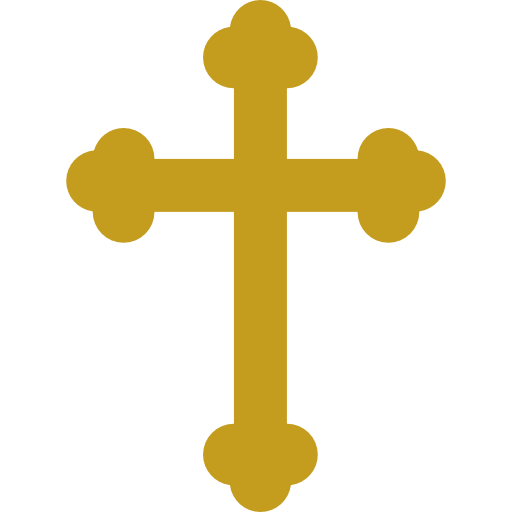
\includegraphics[scale=0.2]{assets/cross.png}\quad
  \textit{Novena a \textbf{Nossa Senhora d'Abadia}}
}
\fancyfoot[RO,RE]{\thepage}

\begin{document}

\subsection*{Novena a Nossa Senhora d'Abadia}

\say{
Celebrar a Festa da Assunção de Maria, mesmo com o nome de Nossa Senhora da Abadia, é afirmar sua participação no mistério da ressurreição, realidade essa como caminho e destino para todos nós. É a consequência, e a justa recompensa dada por Deus, pelo esforço que a pessoa faz para viver a fé na convivência comunitária. O fundamental é ter coração mariano para o encontro com Cristo. 
}

--- Dom Paulo Mendes Peixoto, Arcebispo de Uberaba (MG)

\par\noindent\rule{\textwidth}{0.4pt}

\tableofcontents
\thispagestyle{empty}

% --- Vida / Origem da Novena ---
\newpage

\section{Origem da Devoção}

Nossa Senhora da Abadia é um dos títulos da Virgem Maria. Esta invocação a Maria também é conhecida como Santa Maria do Bouro, pois se originou no Mosteiro (ou Abadia) do Bouro, próximo à cidade de Braga, em Portugal.

\subsection{A imagem de Nossa Senhora da Abadia}

A imagem de Nossa Senhora da Abadia representa Maria de pé, segurando nos braços o menino Jesus, que tem uma coroa na cabeça. Maria veste uma túnica branca com flores de cor rosa e azul. Um cinto vermelho passa por sua cintura. Por cima, um manto azul decorado com belas flores completa sua vestimenta. Na mão direita, Maria segura um cetro para guiar os seus filhos. Na cabeça, ela tem uma linda coroa.

\subsection{Devoção a Nossa Senhora da Abadia}

A devoção a Nossa Senhora da Abadia é muito antiga. Ela pertenceu a uma abadia (mosteiro cujo superior é um abade), conhecida como Mosteiro das Montanhas, que ficava na região do Bouro por volta do ano 883. Quando os muçulmanos invadiram Espanha e Portugal, os monges fugiram e esconderam a imagem da Santa. Muito tempo passou.

\subsection{Redescoberta}

Mais tarde, por volta do ano 1100, um nobre ancião da corte portuguesa, chamado Pelágio Amado recebeu a graça da conversão. Ele abandonou sua vida de riquezas na corte e foi para a Ermida de São Miguel, perto de Braga. Lá ele viveu com um velho eremita que já vivia ali há muitos anos. Certa noite, os dois viram uma luz diferente que vinha do meio de um vale perto de onde estavam. Na noite seguinte o fato se repetiu. Então, os dois resolveram ir até o local quando se fez dia, para ver o que poderia estar fazendo brilhar aquela luz. Foi então que  eles encontraram imagem de Nossa Senhora da Abadia escondida no meio das pedras. Os dois se prostraram agradecendo por esta graça tão especial.

\subsection{A devoção recomeça}

Por causa da redescoberta, os dois eremitas mudaram o casebre em que viviam para o local onde encontraram a Santa. Lá, eles ergueram uma pequena e rústica capela e colocaram a imagem de Nossa Senhora da Abadia. A notícia da descoberta correu e chegou aos ouvidos do arcebispo de Braga. Este foi visitar o local e, depois de ver a pobreza em que os dois eremitas viviam, mandou construir ali uma igreja de pedra lavrada, digna de abrigar os dois santos e a imagem de Nossa Senhora. Aos poucos, outros eremitas se uniram aos dois e a fama dos milagres de Nossa Senhora da Abadia se espalhou em Portugal. Peregrinações começaram a acontecer. Fiéis de todos os cantos vinham rezar, pedir e agradecer pelas graças alcançadas. D. Afonso Henriques, rei de Portugal, foi visitar o santuário e deixou ali uma grande doação para o culto e as necessidades daqueles servos de Deus.

\subsection{A devoção chega ao Brasil}

A devoção a Nossa Senhora da Abadia chegou ao Brasil através dos portugueses e se instalaram primeiramente na região do Triângulo Mineiro. Nessa região, várias cidades têm como Padroeira Nossa Senhora da Abadia. Com o tempo, a devoção passou para Goiás, principalmente em Muquém e na antiga capital, Vila Boa, que ainda conserva sua Igreja Matriz, construída no século XVIII. Atualmente um dos locais mais famosos pelas romarias é o de Nossa Senhora da Abadia da Água Suja, antigo centro de garimpagem de diamantes. O Santuário de Nossa Senhora da Abadia atrai todos os anos, no dia 15 de agosto, um grande número de devotos e a procissão é famosa. Em Uberaba também é grande a devoção a nossa Senhora da Abadia.

\newpage

% --- Orações Diárias ---
\section{Novena de Nossa Senhora d'Abadia}
\subsection*{Oração para todos os dias}

Ó Senhora da Abadia, aqui estão os vossos filhos que, cheios de gratidão, vieram vos agradecer: agradecer o Dom da vida; agradecer o Dom da fé; agradecer a vida divina; agradecer a vida de família e de amizades; agradecer a vida da Igreja; agradecer os cem anos de celebração desta festa.

Estes vossos filhos, Senhora e Mãe, vieram também pedir e suplicar: \\
-- olhai, ó Mãe, estes vossos filhos e suas famílias; \\
-- olhai, ó Mãe, esta Paróquia e seu Vigário; \\
-- olhai, ó Mãe, esta diocese e seus Bispos; \\
-- olhai, ó Mãe, a Igreja e o Santo Padre, o Papa. 

Fazei, ó Mãe e Rainha, que estes vossos filhos sejam testemunhas das verdades libertadoras anunciadas no Evangelho de vosso filho Jesus realizando o seu reino também na terra.

Ó Mãe, estes filhos querem gozar um dia de vossa presença na glória do céu, onde de corpo e alma estais com o Pai, reinais com vosso Filho Jesus e viveis com o Espírito Santo. Amém. 


\[
  \textbf{Pai-Nosso, Ave-Maria, Glória Ao Pai.}
\]

\response. \quad Roga por nós, Milagrosa Nossa Senhora d'Abadia!

\versicle. \quad Para que nos tornemos dignos das promessas de Cristo. \\




\textbf{Oremos:} Ó Deus, que pela imagem milagrosa de tua Mãe em Sinj mostraste o poder salvador de teu amor, faze-nos dignos de amá-la sinceramente e, por sua intercessão, chegar a ti, que vives e reinas pelos séculos dos séculos. Amém!


\vfill

\begin{center}
\subsection*{Fontes:}
História adaptada de: \underline{\href{https://cruzterrasanta.com.br/historia-de-nossa-senhora-abadia/20/102/}{Cruz Terra Santa}}\\ 
Novena Adaptada: \underline{\href{https://oracoes.pt/novena-a-nossa-senhora-de-sinjska/}{ORACOES.PT}}
\end{center}


\end{document}
